\section{Introduction}
\ap{2 Pages for: Introduction + Motivating Examples + Rel. work}

\ap{The architectural difference btw Bmv2 and Tofino. Processing pipeline, CP, etc.}

Motivation/ introduction:
\begin{itemize}
    \item Network verification is important as softwarization of the data plane is getting more and more attention in research as well as the industry
    \item because network outages are costly and small errors can lead to whole network outages
    \item existing verification approaches are not sufficient
    % should the next points with hint on why existing work is insufficient be here already? or is it better to fully move that to related work?
    \item existing approaches can already capture few kinds of bugs but are either based on symbolic execution, which is suffering from path explosion problem if the program is branchy
    \item and/or assume a lot of additional manual work to reflect expected program behaviour
    \item so these approaches are either lacking possibilities to also verify large or branchy programs but also require manual work even if the programs to be verified implement the same high level logic, e.g. layer 3 packet processing.
    \item Problem statement: Can the correctness of P4 programs be automatically verified?
    \item this paper aims at using radically different approaches changing the game of network verification and providing a solution to automatically verify P4 programs for a wide variety of common bugs in P4 programs.
    \item contributions: 
    \item implement reinforcement learning assisted fuzzing framework/ approach to automatically verify P4 programs overcoming several limitations of existing work.
    
\end{itemize}
\section{Motivating Examples}
\ap{draw clean diagrams in pdf using google presenation with scenarios just like in PAZZ which P4v, Vera, ASSERT etc cannot detect}

\begin{figure}[tp]
\centering
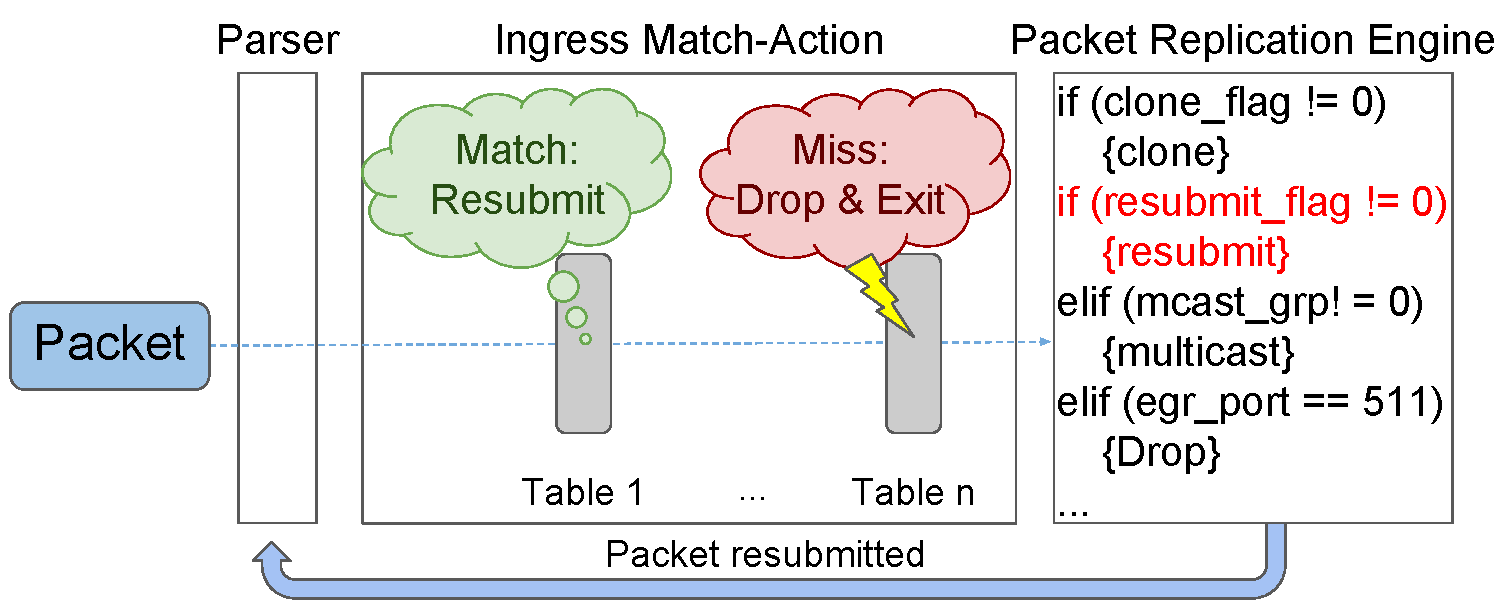
\includegraphics[width=\linewidth]{figures/scenario_v5.pdf}
\caption{Example of Target Specific Drop} %\ap{Font looks too small so make sure it is readable by naked eye. Use clker.com for free images which are not copyright}
\end{figure}
Example scenario:
\begin{itemize}
    \item After Packet traversed the parser it is processed in ingress processing
    \item during ingress processing tables are applied
    \item if e.g. a packet is matched in a table and as a result a resubmit action is executed, the resubmit flag for that packet will be set (part of the metadata)
    \item if in a later stage the packet is marked for drop and ingress processing is aborted, e.g. miss in ACL table, the packet reaches the packet replication engine (PRE).
    \item The architecture/target specific implementation defines what happens with such a packet. In Bmv2 with simple switch target (standard target from tutorials), the packet would be resubmitted even though the programmer would expect it to be dropped.(see figure)
\end{itemize}

Verification approaches and comparison (or should that be part of related work?) Or only introducing Fuzzing?
\begin{itemize}
    \item Fuzzing is ...
    \item types of fuzzing (White-box, grey-box, black-box, dumb, smart, generation based, mutation based, ...?)
    \item
\end{itemize}
quick intro on machine learning/ reinforcement learning
\begin{itemize}
    \item What is machine learning?
    \item taxonomy
    \item reinforcement learning
    \item Q learning
    \item deep Q learning
    \item usually used to let computers learn to play games (maybe ref. Google Deepmind papers as examples)
\end{itemize}

